\documentclass[a4paper,french]{article}
\usepackage[utf8]{inputenc}
\usepackage{graphicx}
\usepackage[left=2cm,right=2cm,top=2cm,bottom=2cm]{geometry}
\usepackage{babel}
\setlength{\parindent}{20pt}

\begin{document}
	\Large
	PRIN Guillaume \hfill Année 2015-2016\newline
	\begin{center}
		\Huge
		Projet : Génération de dégradations physiques sur les modèles 3D
	\end{center}
	\vspace*{2cm}
	\begin{center}
		\Huge
		\underline{Rapport de projet}
	\end{center}
	\begin{center}
	
\includegraphics
	{ulco.png}
	\end{center}
	\vfill
	Tuteurs de projet : 
	\begin{itemize}
		\item Christophe Renaud
		\item François Rousselle
	\end{itemize}
	\newpage
	\tableofcontents
	\newpage
	\section{Positionnement du projet}
		\subsection{Rappel : Contexte et définition du problème}
			Dans le cadre de reconstitutions virtuelles historiques,  le challenge de l'équipe pluridisciplinaire réunie (informaticiens et historiens) consiste à s'approcher au plus près de la réalité historique de l'environnement reconstruit. Au travers de recherches approfondies dans divers fonds d'archives, les historiens apportent ainsi des connaissances fondamentales à la reconstruction 3D des environnements ciblés, permettant ensuite une visualisation plus ou moins réaliste et/ou plus ou moins interactive de ces environnements, pour des applications diverses à destination des chercheurs ou du grand public.. \par
			Un défaut fréquent de ces reconstitutions réside dans le fait qu'ils apparaissent comme neufs, ce qui est clairement préjudiciable à leur interprétation dans leur contexte historique. Un travail complémentaire, effectué par des infographistes, consiste alors à introduire des dégradations dans ces environnements, provenant tant de causes naturelles (vent, pluie, etc.) que humaines (usures dues aux passages répétés, chocs, déprédations volontaires, etc.). \par
			L'objectif de ce projet est de se focaliser sur un type particulier de dégradation, lié à l'usure et aux chocs reçus par les pierres qui apparaissent dans le bâti reconstruit, qu'il s'agisse de marches d'escalier ou des pierres des murs. Le travail à réaliser consistera à développer le code d'une méthode existante et à tester son utilisation dans le cadre d'une reconstitution du Pont Notre Dame en 1720.
		\subsection{Encadrants}
			Je suis encadré pendant ce projet par M. Christophe Renaud, directeur du LISIC et responsable de l'équipe IMAP (Images et Apprentissage) du laboratoire de recherche, et par M. Rousselle, maître de conférences, enseignant-chercheur à l'IUT de Calais-Boulogne, et membre de l'équipe IMAP du laboratoire de recherche.
		\subsection{L'état initial}
			Le pont Notre Dame a déjà été intégralement modélisé sous 3DsMax par M. Rousselle, et m'a été fourni au format Wavefront obj à des fins de tests. 
		\subsection{Durée du projet}
			La période libre de projet s'étale du 18 avril au 05 juin 2016. Toutefois, comme mentionné par M. Fabien Teytaud, responsable du Master 1 Informatique ISIDIS, il est fort recommandé de commencer le projet dès le mois de janvier.
		\subsection{Les outils mis en place}
			Une boite de dépôt github a été créée pour l'occasion, à l'adresse suivante :  https://github.com/guil-prin/notreDame . Régulièrement mise à jour, vous pouvez y trouver l'évolution du développement (dossier "dev"), les documents produits pour le projet (dont ce rapport, dans le dossier "documentation"), et les sources finales (dossier "sources"). Les descriptions fonctionnelles du projet sont d'ailleurs dans le cahier des charges fourni le 25 avril. \par
			Un disque dur avec un système d'exploitation Debian vierge installé m'a été gracieusement prêté par Nathalie Ramat, responsable du parc informatique de l'ULCO, afin que je puisse bénéficier du statut d'administrateur sur mon pc, et que je puisse donc installer les outils nécessaires au développement du projet. \par
			Une bibliothèque c++ a aussi été mise en place : CGAL. Disponible sur le site http://www.cgal.org/, elle permet de travailler sur une structure 3D avec des outils fournis pour définir un objet 3D et ses composants (arêtes, sommets, faces). La recherche de cette bibliothèque a été une partie du travail préliminaire au projet.
		\newpage
	\section{Travaux préliminaires}
		\subsection{Étude documentaire}
			Deux notes de recherche m'ont été confiés par M. Renaud lors de notre premier entretien : 
				\begin{itemize}
					\item Surface Aging by Impacts \cite{PPD01}
					\item Modeling cracks and fractures \cite{Liris-6004}
				\end{itemize}\par
			Il m'a aussi expliqué le but du projet : le modèle 3D déjà créé est terminé, mais il s'avère être "trop beau" par rapport à la réalité. En effet, les bâtiments modélisés s'avèrent en réalité avoir environ une centaine d'années d'après les historiens avec qui ils travaillent. Le but est donc de vieillir le modèle 3D afin de le prendre plus proche de la réalité. \par
			Il m'a donc été demandé à ce moment de consulter ces papiers de recherche, et plus particulièrement Surface Aging by Impacts \cite{PPD01}. J'ai eu plusieurs réunions avec M. Rousselle pour discuter de ce papier en détail. J'ai eu, à la demande de ce dernier, à réaliser une synthèse personnelle de ce papier afin de me faire comprendre la démarche d'un document scientifique (un cours d'initiation à la recherche a été enseigné par M. Verel à ce propos, mais n'a eu lieu que après cette réunion). Cette synthèse est disponible dans le dossier documentation du projet. \par
			Une troisième note de recherche me sera fournie au début de la période de projet, Real-Time Relief Mapping on Arbitrary Polygonal Surfaces \cite{Policarpo:2005:RRM:1053427.1053453}. Bien que consultée, elle ne sera pas intéressante pour cette période de projet.
			
		\subsection{Recherche de bibliothèques}
			Au cours de ces entretiens, il m'a aussi été demandé de rechercher des bibliothèques c++ afin d'éviter à devoir tout coder. En effet, la modélisation 3D est un domaine extrêmement en vogue à l'heure actuelle (que ce soit pour des simulations historiques, des modélisations de prototypes, des créations de jeux vidéos, ...), et de nombreuses personnes ont déjà travaillé dans ce domaine. Deux bibliothèques ont ainsi été trouvées par mes soins : les bibliothèques Assimp (http://www.assimp.org/) et Magnum (http://mosra.cz/blog/magnum.php), don la dernière n'a pas retenu notre attention. par la suite, M. Rousselle s'est rappelé d'un projet graphique réalisé quelques années auparavant par deux anciens étudiants, et ils avaient utilisé la bibliothèque CGAL. Cette dernière répondant à nos besoins, elle a été gardée pour le développement, tout en mettant de côté Assimp s'il s'avère que CGAL montre des limites. 
		\newpage
		
	\section{Recherche et Développement}
		\subsection{Structure d'un objet 3D}
			Un objet 3D est défini via la bibliothèque CGAL comme un Polyhedron\_3 composé de faces, arêtes, sommets, et de relations entre ces composants. Chacune de ses arêtes est composé de deux demi-arêtes (halfedge), ayant chacun un sens opposé à l'autre. Les relations entre ces composants peut se définir de la manière comme représenté dans la Figure 1. \par 
			Il est ainsi possible d'accéder à partir d'un composant à tous les autres composants adjacents. Par exemple, halfedge()-\textgreater facet() permet d'accéder dans cette figure à la face qui contient la demi-arête en rouge.
			\begin{figure}
				\centering
				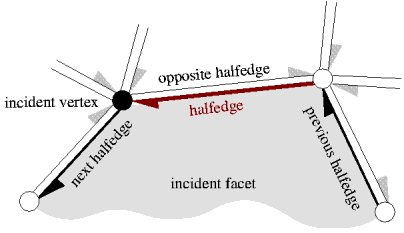
\includegraphics
				{halfedge_small.png}
				\caption{Structure d'un polyhedron}
			\end{figure}
		\subsection{Chargement d'un obj}
			Le premier obstacle a été de gérer le chargement d'un fichier de format obj et de le transcrire comme un Polyhedron\_3. En effet, CGAL ne gère pas nativement cette option, ayant préféré le format .off. Cependant, un développeur nommé James Greggson a publié sur son blog (http://jamesgregson.blogspot.fr) en mai 2012 une version de loader obj et transcrit en Polyhedron\_3. J'ai donc repris son code et l'ait amélioré pour gérer en plus la subdivision en plusieurs Polyhedrons s'il s'avère qu'un fichier .obj contenait plusieurs objets en eux-même (la version initiale du développeur chargeait tous les objets d'un fichier obj en un seul Polyhedron\_3). 
		
		\subsection{Exporter un obj}
			De la même manière, il m'a fallu récupérer le fichier obj une fois le traitement du Polyhedron terminé. Étrangement, là où CGAL n'a pas prévu un chargeur obj, il a prévu un enregistreur, avec la fonction print\_polyhedron\_wavefront(). Il suffit juste d'exporter les Polyhedron un par un dans un même fichier, et on récupère ainsi un fichier obj prêt à l'emploi (pour le consulter via un logiciel adapté, comme Blender).
		
	\newpage
\bibliographystyle{alpha}
\bibliography{biblio}
		
\end{document}

